\chapter{Appendix}

\section{Variations for signal strength visualization over time}
\label{appendix_signal_strength}

This section contains various visualizations for different users' scanned access
points over time. On the x axis we have the time frame, while on the y axis we
have the signal strength for the identified access points. The legend presents
only the top $10$ predominant access points (which have appeared the most
during scans), however the plot displays all access points. The figures are
Fig.~\ref{user_6_cross_1d}, Fig.\ref{user_6_star_1d},
Fig.~\ref{user_6_cross_line_1d}, Fig.\ref{user_6_o_line_1d}.

\begin{figure}[h]
\centering
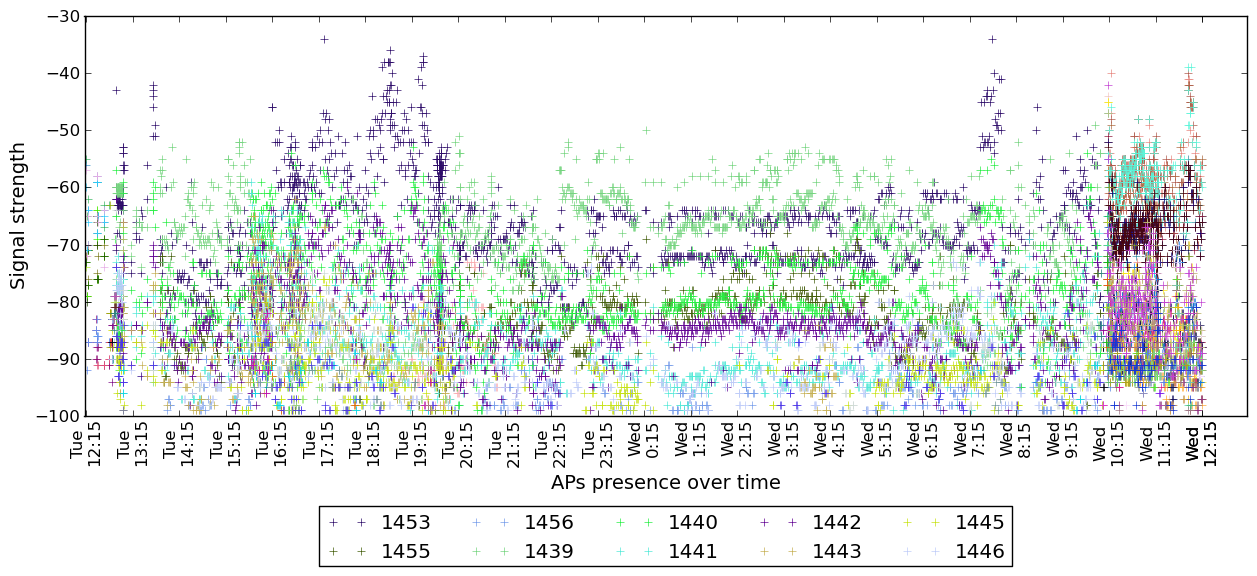
\includegraphics[height =
0.45\textwidth]{figures/cros_user_6_sorted_1days_plot.png}
\caption{Example of the APs registered for an user throughout one day with
``+'' markers}
\label{user_6_cross_1d}
\end{figure}

\begin{figure}[h]
\centering
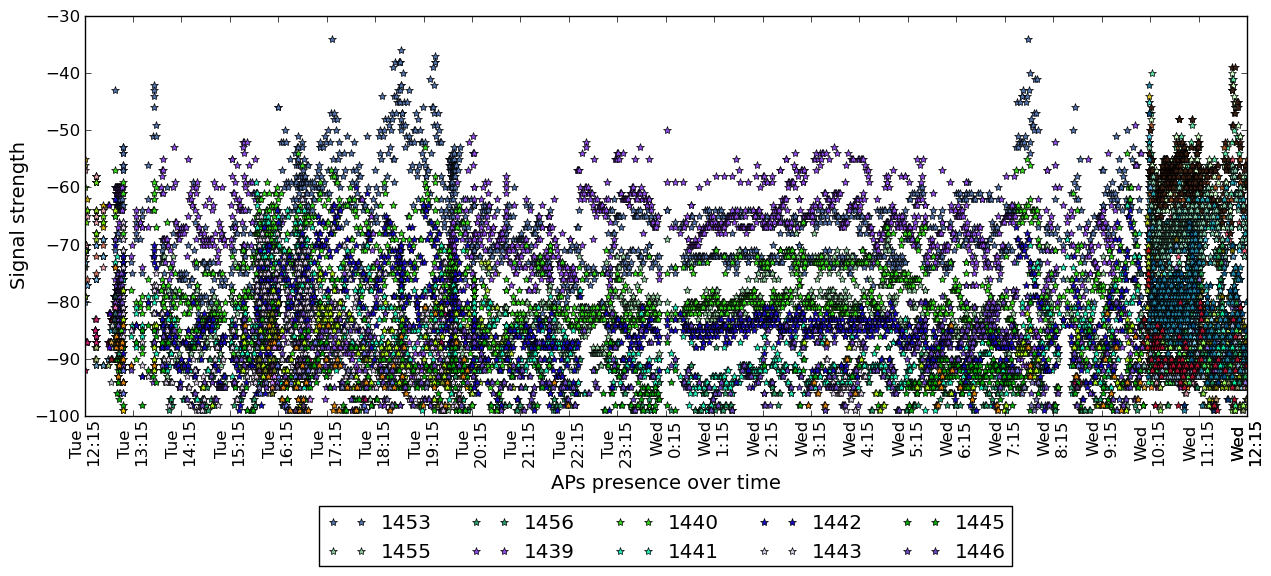
\includegraphics[height =
0.45\textwidth]{figures/star_user_6_sorted_1days_plot.png}
\caption{Example of the APs registered for an user throughout one day with
``*'' markers}
\label{user_6_star_1d}
\end{figure}

\begin{figure}[h]
\centering
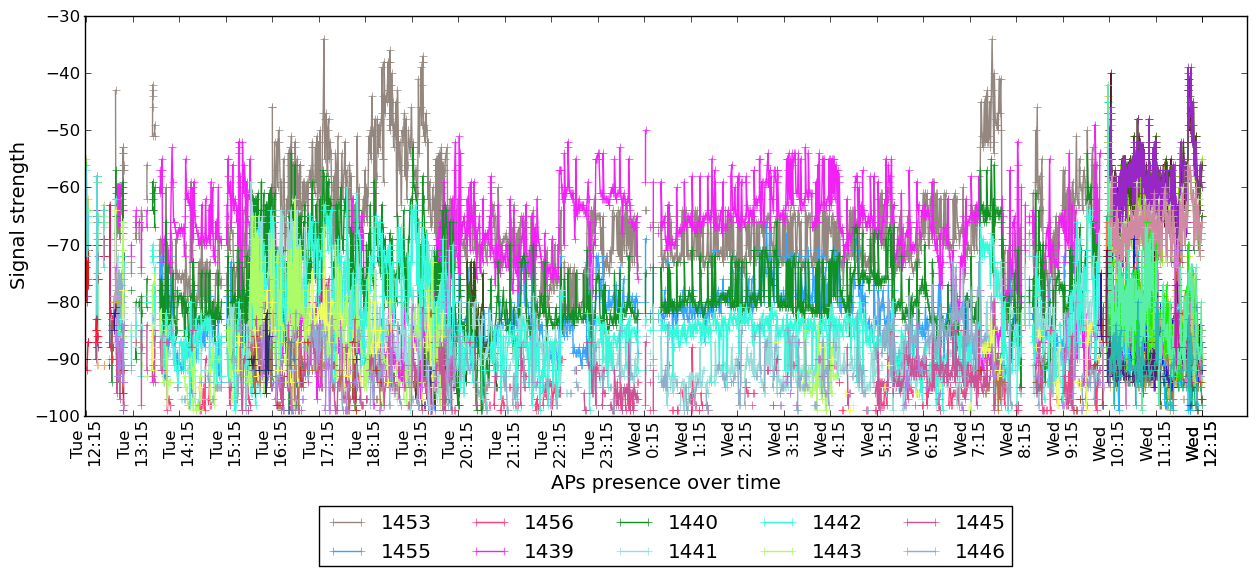
\includegraphics[height =
0.45\textwidth]{figures/cros_line_user_6_sorted_1days_plot.png}
\caption{Example of the APs registered for an user throughout one day with
``+'' and line markers}
\label{user_6_cross_line_1d}
\end{figure}

\begin{figure}[h]
\centering
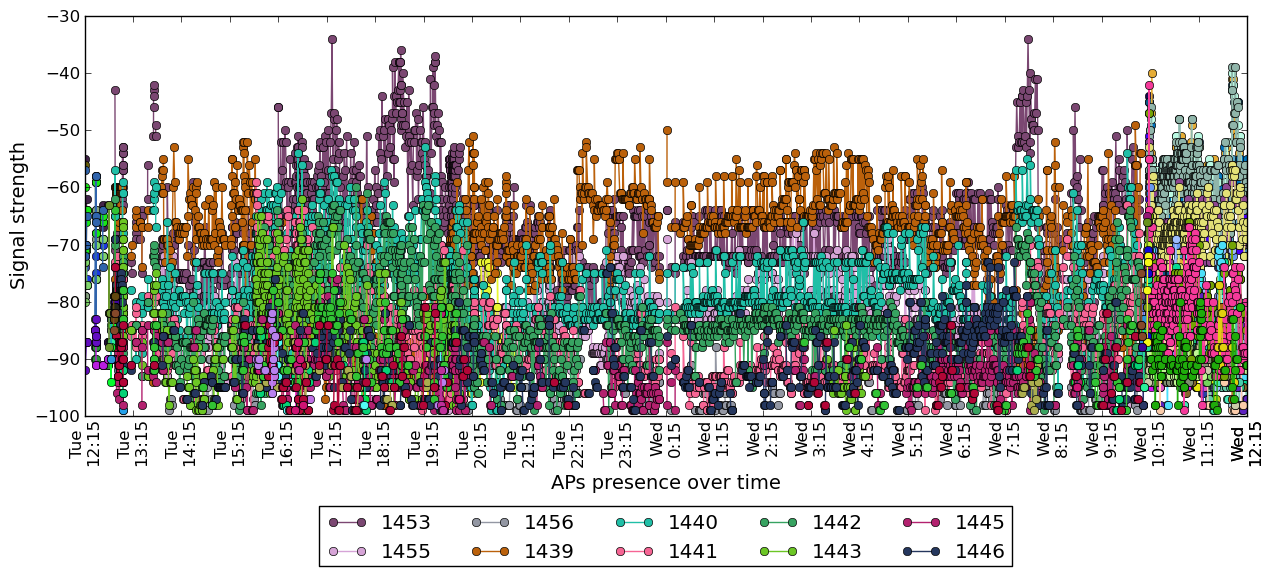
\includegraphics[height =
0.45\textwidth]{figures/o_line_user_6_sorted_1days_plot.png}
\caption{Example of the APs registered for an user throughout one day with
``o'' and line markers}
\label{user_6_o_line_1d}
\end{figure}

\section{Sample density for APs identified for a user}
\label{appendix_sample_density}

This section contains the visualization for the signal strength of the APs
identified as being associated to a user throughout $3$ days as well as the
sample density for the top $10$ predominant APs throughout this time.

\begin{figure}[h]
	\centering
	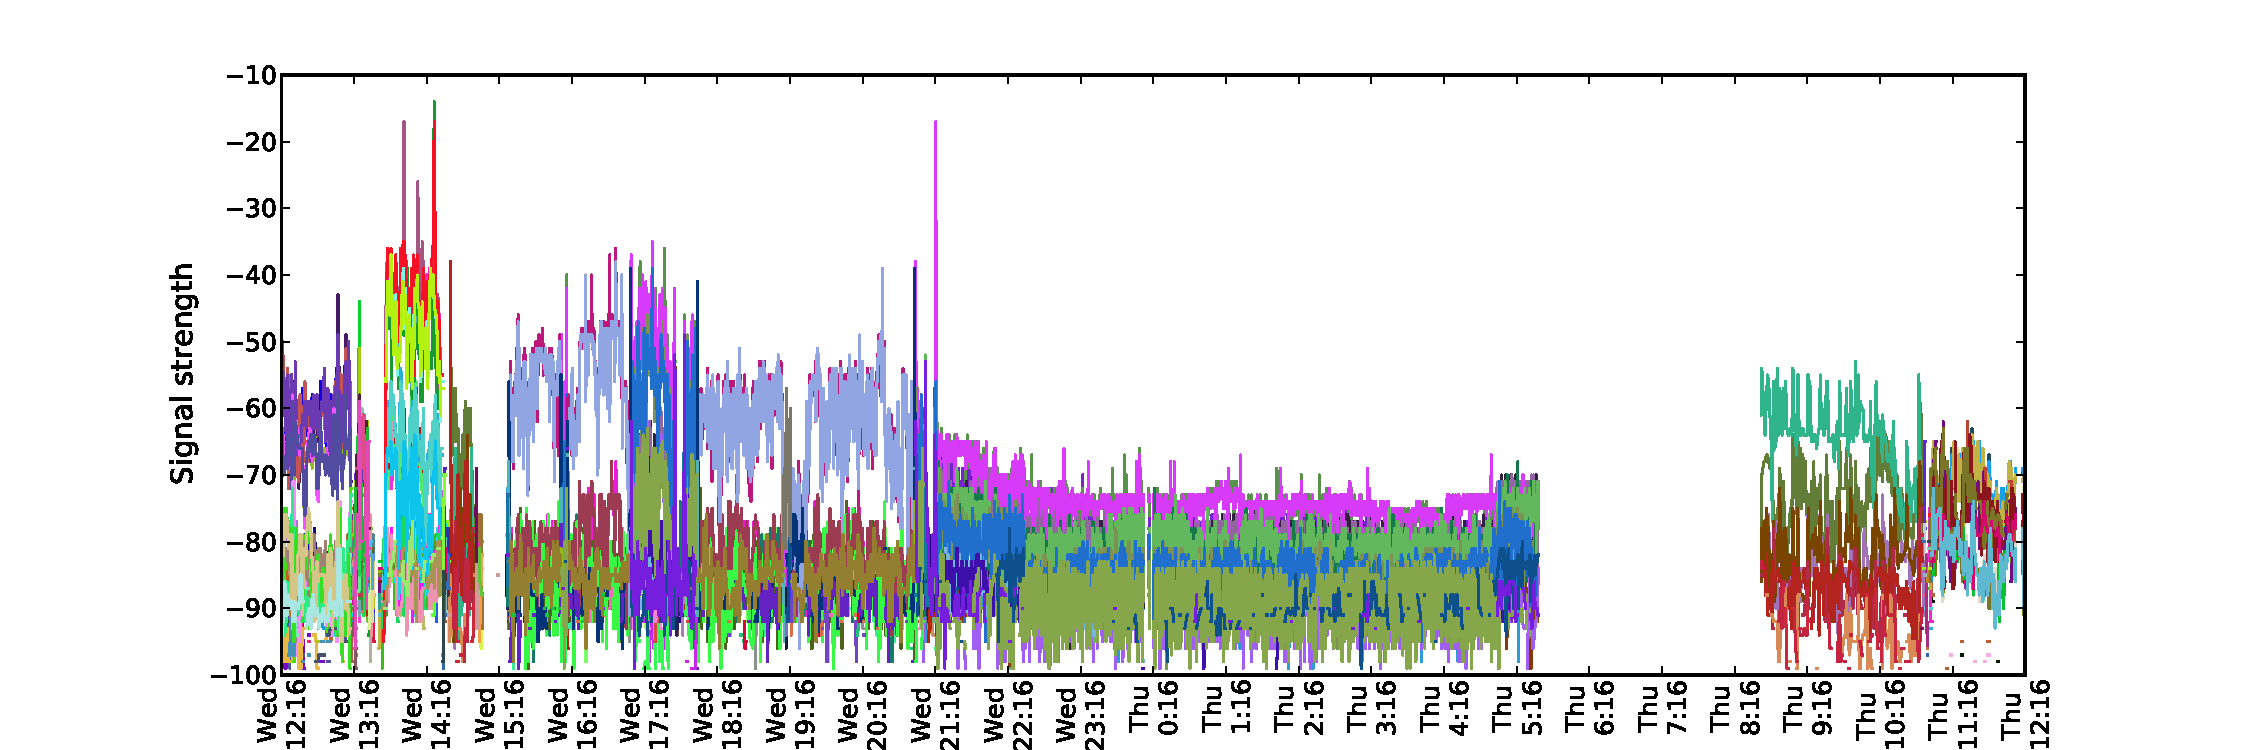
\includegraphics[width=12cm,height=6cm,keepaspectratio]{figures/complete_on_bssid15181_for_1.split/complete_on_bssid15181_for_1_1.pdf}
	\caption{Signal strength visualization}
	\label{fig:rssi_6_2nd_day}
\end{figure}
\begin{figure}[h]
	%\centering
	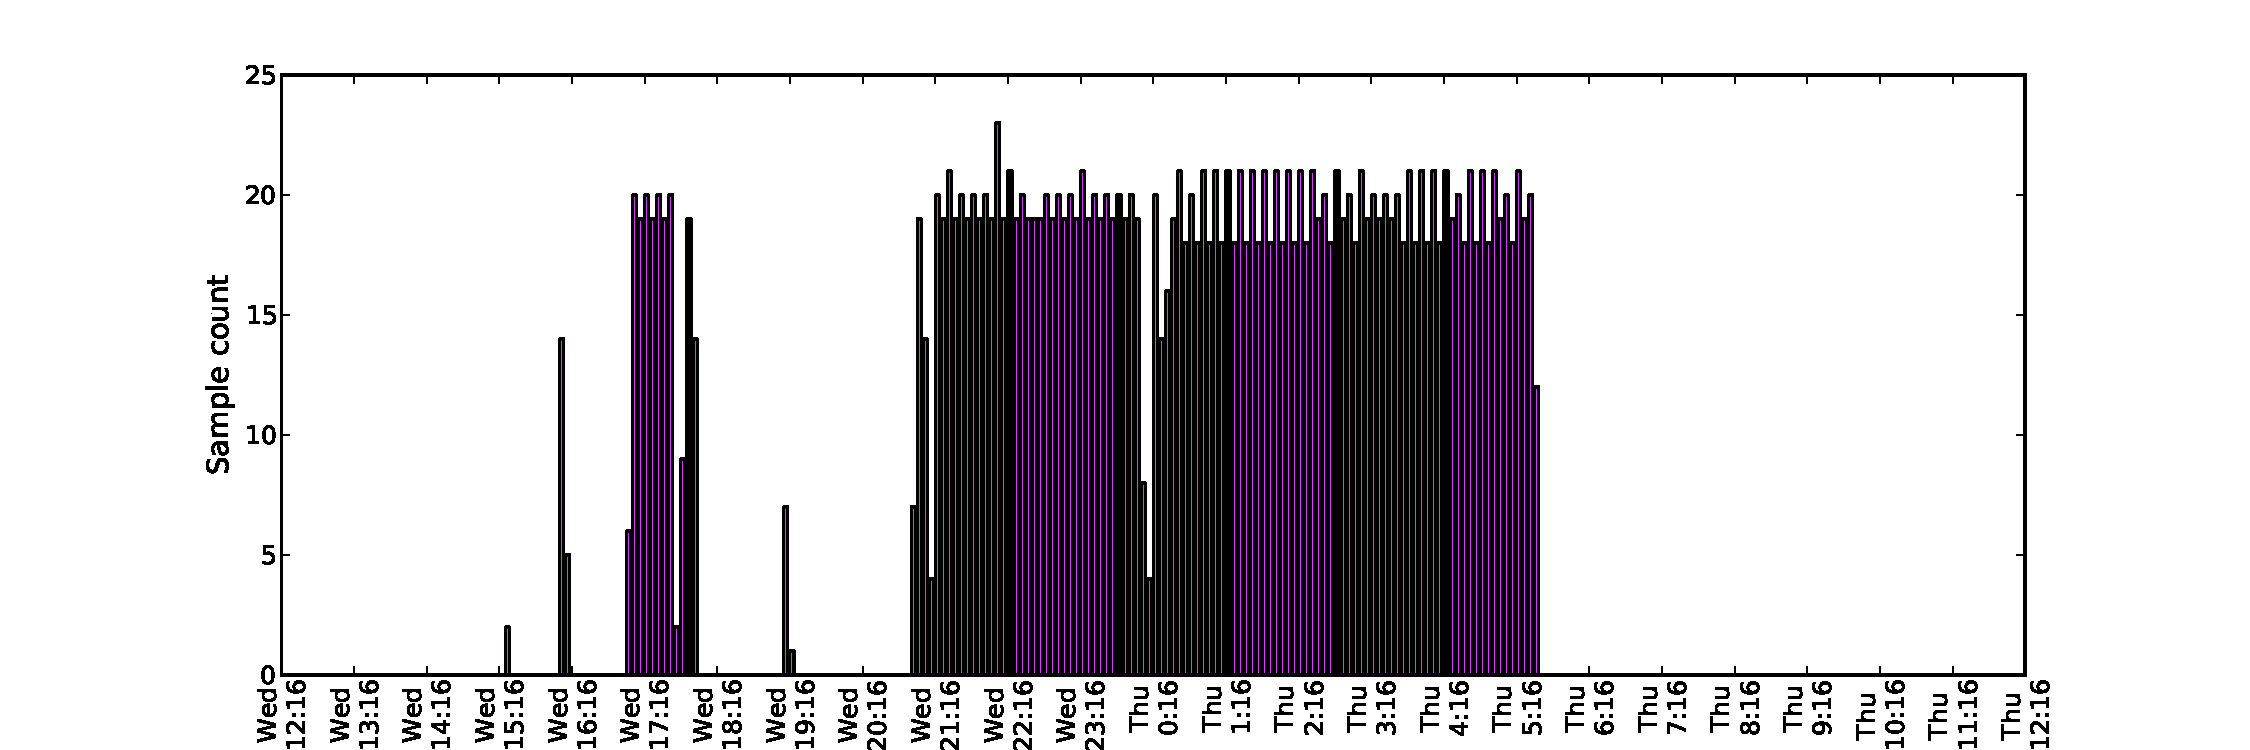
\includegraphics[width=12cm,height=6cm,keepaspectratio]{figures/complete_on_bssid15181_for_1.split/complete_on_bssid15181_for_1_2.pdf}
	\caption{Sample density for AP identified with 15181}
	\label{samples_6_2nd_day}
\end{figure}

\subsection{Average signal strength for APs identified for a user}
\label{appendix_avg_signal}

This section contains the visualization for the signal strength of the APs
identified as being associated to a user throughout $3$ days as well as the
average signal for the top $10$ predominant APs calculated for a consecutive $5$
minutes time windows throughout the $3$ days.

\subsection{Running average signal strength}
\subsection{Signal presence}